\documentclass{article}
\usepackage[utf8]{inputenc}
\usepackage{listings}
\usepackage{cite}
\usepackage{amsmath,amssymb,amsfonts}
\usepackage{algorithmic}
\usepackage{graphicx}
\usepackage{textcomp}
\usepackage{xcolor}
\usepackage{color}
\usepackage{url}
\definecolor{dkgreen}{rgb}{0,0.6,0}
\definecolor{gray}{rgb}{0.5,0.5,0.5}
\definecolor{mauve}{rgb}{0.58,0,0.82}
\lstset{%
    aboveskip=3mm, belowskip=3mm,
    showstringspaces=false,
    columns=flexible,
    basicstyle={\small\ttfamily},
    numbers=none,
    numberstyle=\tiny\color{red},
    keywordstyle=\color{blue},
    commentstyle=\color{dkgreen},
    stringstyle=\color{mauve},
    breaklines=true,
    breakatwhitespace=true,
    tabsize=3
}

\newcommand{\code}[1]{\texttt{#1}}
\newcommand{\val}[1]{#1_{\text{val}}}
\newcommand{\est}[1]{#1_{\text{est}}}

\begin{document}
\title{Lab 1 --- Supervised learning}
\author{Malcolm Vigren, \textit{malvi108} \\
        Emil Segerbäck, \textit{emise935}}

\maketitle

\section{Overview}
Dataset 1 can be classified using a linear classifier. However, the
other datasets are not linearly separable, so they need to be classified
using a non-linear classifier.

\section{Downsampling}
Downsampling the data removes noise and distorsions from the images,
which prevents the network from trying to learn the noise.

\section{kNN}
The \texttt{mink} function in matlab was used to find the closest $k$
data points and then \texttt{mode} was used to check for the most
frequent kind.

\subsection{Draws in kNN}
Because \texttt{mode} returns the smallest element in a case of a tie,
that is also what happens in this algorithm.

\section{Selection of best $k$}
For each value of $k$ between 0 and 100, the dataset was evaluated and
accuracy calculated. The accuracies were then plotted as a function
of $k$, and the $k$ that gave the highest accuracy was selected.

\subsection{Dataset 1}

Cross-validation, as shown in Figure~\ref{fig:cv1}, showed in this
case that k = 4 was optimal, giving an accuracy of 98.5\%. 
The result of kNN with this $k$ is shown in Figure~\ref{fig:knn1}.

\begin{figure}[h!]
    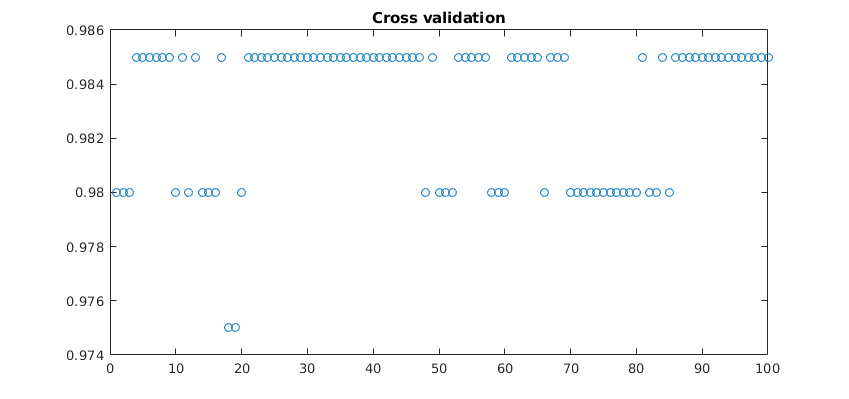
\includegraphics[width=13cm]{dataset1knncv.png}
    \caption{kNN cross-validation of dataset 1}
    \label{fig:cv1}
\end{figure}

\begin{figure}[h!]
    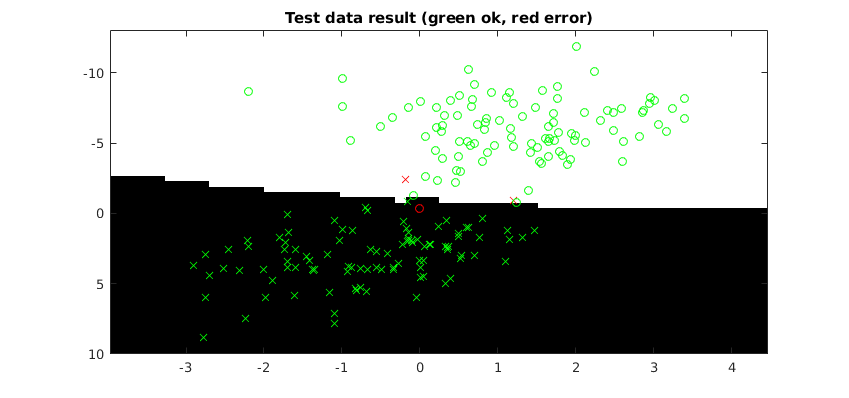
\includegraphics[width=13cm]{dataset1knnres.png}
    \caption{kNN result of dataset 1}
    \label{fig:knn1}
\end{figure}

\subsection{Dataset 2}

Cross-validation, as shown in Figure~\ref{fig:cv2}, showed in this
case that k = 1 was optimal, giving an accuracy of 99.5\%. 
The result of kNN with this $k$ is shown in Figure~\ref{fig:knn2}.

\begin{figure}[h!]
    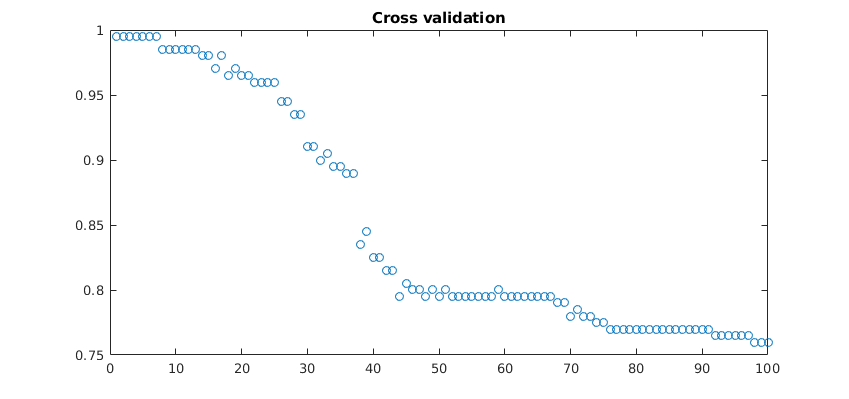
\includegraphics[width=13cm]{dataset2knncv.png}
    \caption{kNN cross-validation of dataset 2}
    \label{fig:cv2}
\end{figure}

\begin{figure}[h!]
    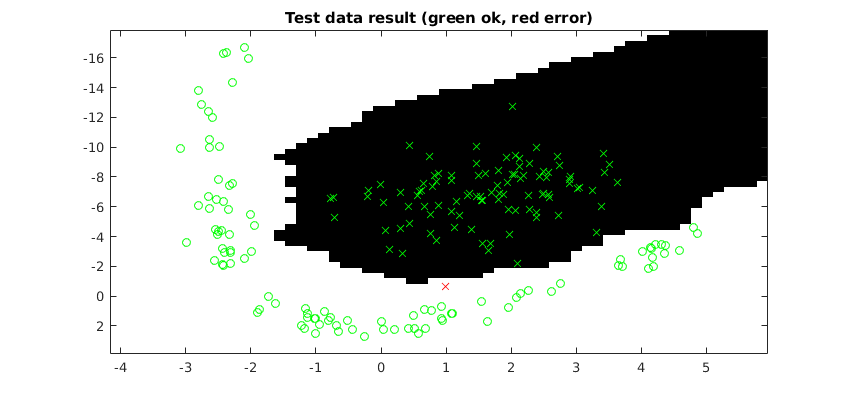
\includegraphics[width=13cm]{dataset2knnres.png}
    \caption{kNN result of dataset 2}
    \label{fig:knn2}
\end{figure}

\subsection{Dataset 3}

Cross-validation, as shown in Figure~\ref{fig:cv3}, showed in this
case that k = 1 was optimal, giving an accuracy of 100\%. 
The result of kNN with this $k$ is shown in Figure~\ref{fig:knn3}.

\begin{figure}[h!]
    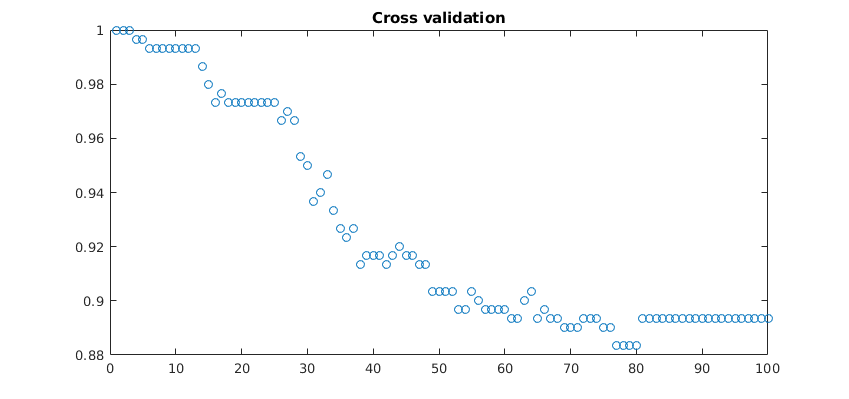
\includegraphics[width=13cm]{dataset3knncv.png}
    \caption{kNN cross-validation of dataset 3}
    \label{fig:cv3}
\end{figure}

\begin{figure}[h!]
    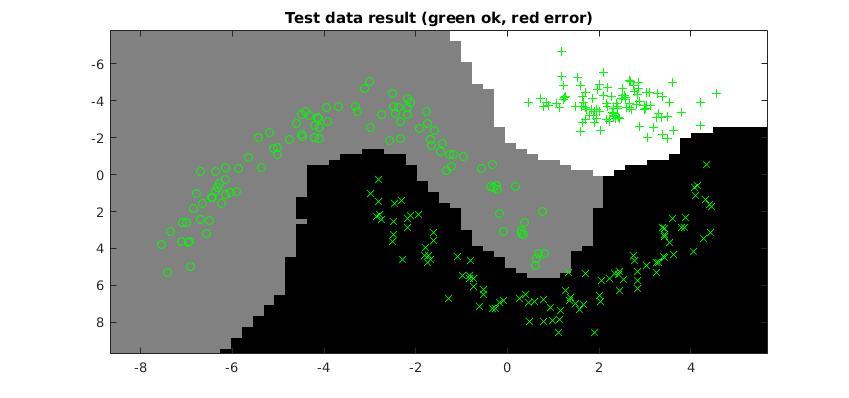
\includegraphics[width=13cm]{dataset3knnres.png}
    \caption{kNN result of dataset 3}
    \label{fig:knn3}
\end{figure}

\subsection{Dataset 4}

Cross-validation, as shown in Figure~\ref{fig:cv4}, showed in this
case that k = 7 was optimal, giving an accuracy of 97.5\%. 
The result of kNN with this $k$ is shown in Figure~\ref{fig:knn4}.

\begin{figure}[h!]
    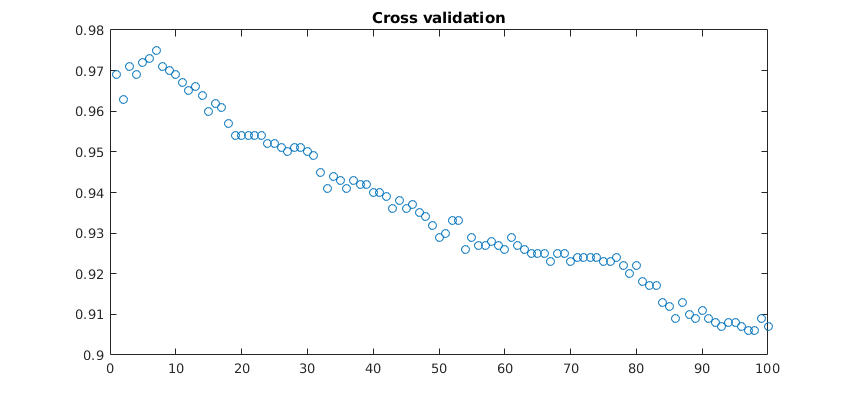
\includegraphics[width=13cm]{dataset4knncv.png}
    \caption{kNN Cross-validation of dataset 4}
    \label{fig:cv4}
\end{figure}

\begin{figure}[h!]
    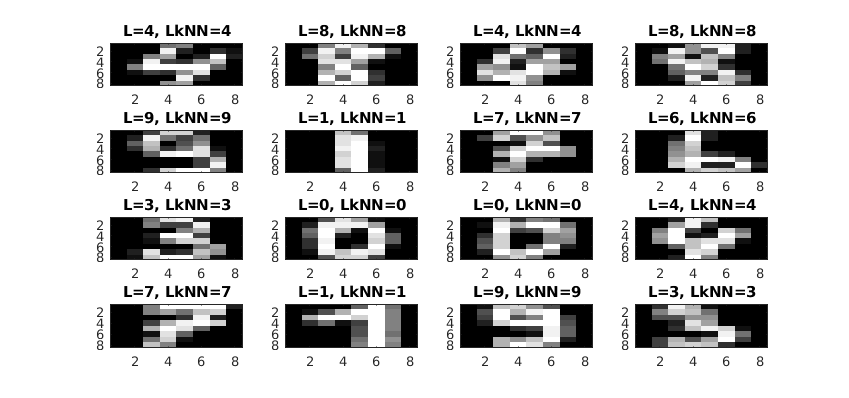
\includegraphics[width=13cm]{dataset4knnres.png}
    \caption{kNN Result of dataset 4}
    \label{fig:knn4}
\end{figure}

\section{Backpropagation}

This section describes how the backpropagation was implemented.

\subsection{Single layer}

The gradient of the cost function was evaluated to

\begin{equation}
  \frac{\partial \epsilon}{\partial w_{ij}} =
  \frac{\partial \epsilon}{\partial z_j}
  \frac{\partial z_j}{\partial s_j}
  \frac{\partial s_j}{\partial w_{ij}}
\end{equation}

where $s_j$ is

\begin{equation}
  s_j = \sum_{k}{w_{kj}h_k}
\end{equation}

and $z_j = s_j$, since we don't use an activation function.
The partial derivatives were evaluated to

\begin{equation}
    \frac{\partial \epsilon}{\partial z_j} = -2(y_j - z_j)
\end{equation}

\begin{equation}
    \frac{\partial z_j}{\partial s_j} = 1
\end{equation}

\begin{equation}
    \frac{\partial s_j}{\partial w_{ij}} = h_i
\end{equation}

\subsection{Multi layer}

The gradient of the weights of the output layer was evaluated as:

\begin{equation}
  \frac{\partial \epsilon}{\partial w_{ij}} =
  \frac{\partial \epsilon}{\partial z_j}
  \frac{\partial z_j}{\partial s_j}
  \frac{\partial s_j}{\partial w_{ij}}
\end{equation}

This is similar to the gradient in the single-layer-network, where $h_i$
in the last partial derivative is replaced with the output from the hidden
layer:

\begin{equation}
    \frac{\partial s_j}{\partial w_{ij}} = \sigma(a_j)
\end{equation}

where $a_j$ is 

\begin{equation}
    a_j = \sum_{n=1}^Q v_{jn}h_n
\end{equation}

The gradient of the hidden layer was evaluated as follows:

\begin{equation}
  \frac{\partial \epsilon}{\partial v_{jn}} =
  \frac{\partial \epsilon}{\partial z_m}
  \frac{\partial z_m}{\partial s_m}
  \frac{\partial s_m}{\partial q_j}
  \frac{\partial q_j}{\partial a_j}
  \frac{\partial a_j}{\partial v_{jn}}
\end{equation}

where $q_j = \sigma(a_j)$.

\section{Training}

This section describes the training of the neural networks, as well as the
results of the training. The parameters were in all cases found through trial
and error, with some guidance of the complexity of the problems and the
plot of the test and training errors.

\subsection{Dataset 1}

We chose the single-layer network for dataset 1, since this is easily
linearly separable. We used 200 iterations and a learning rate of
0.0001. Figure~\ref{fig:res1} shows the result of this.

\begin{figure}[h!]
    \label{fig:res1}
    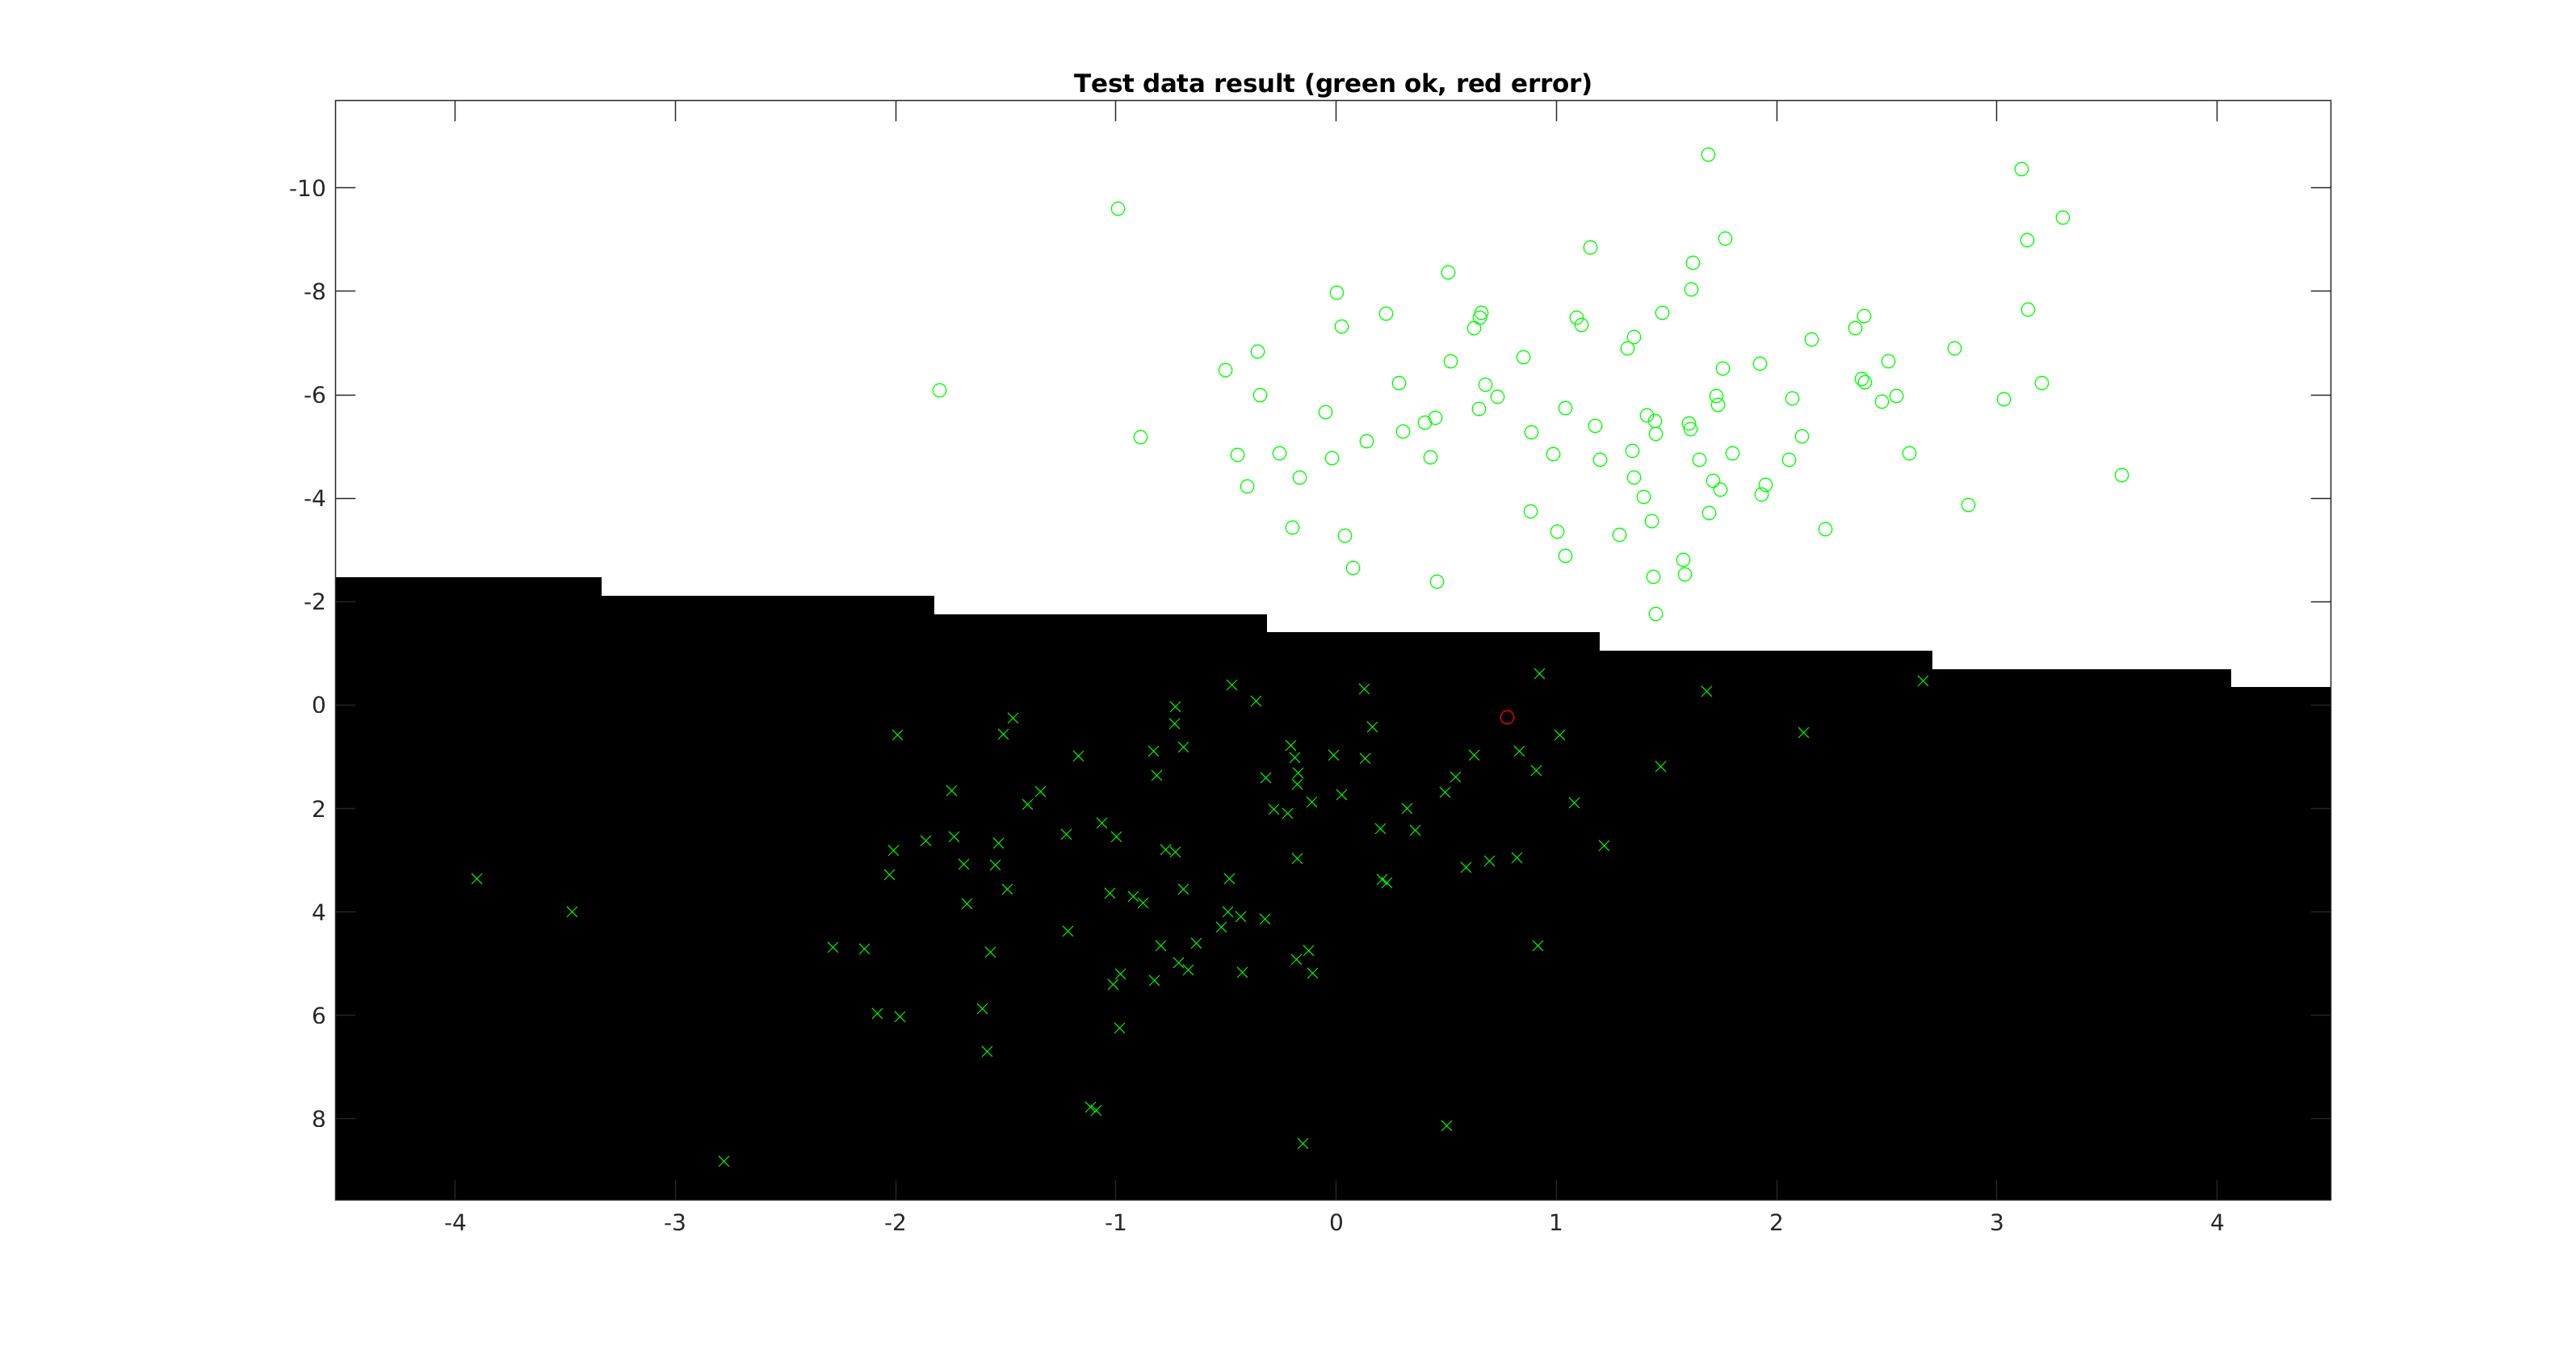
\includegraphics[width=13cm]{dataset1res.png}
    \caption{Results for dataset 1}
\end{figure}

\subsection{Dataset 2}
Here we used a multi-layer network with 10 hidden neurons, 4000 iterations and a
learning rate of 0.002. A multi-layer network is required here, since the data
is not linearly separable with only 2 dimensions. Having more hidden neurons
than input neurons increases the dimensionality of the problem, making it
possible to separate the classes.

The exact parameters were found through trial and error. They were chosen such
that we got high accuracy without taking too long to train.
Figure~\ref{fig:res2} shows the result of this.

\begin{figure}[h!]
    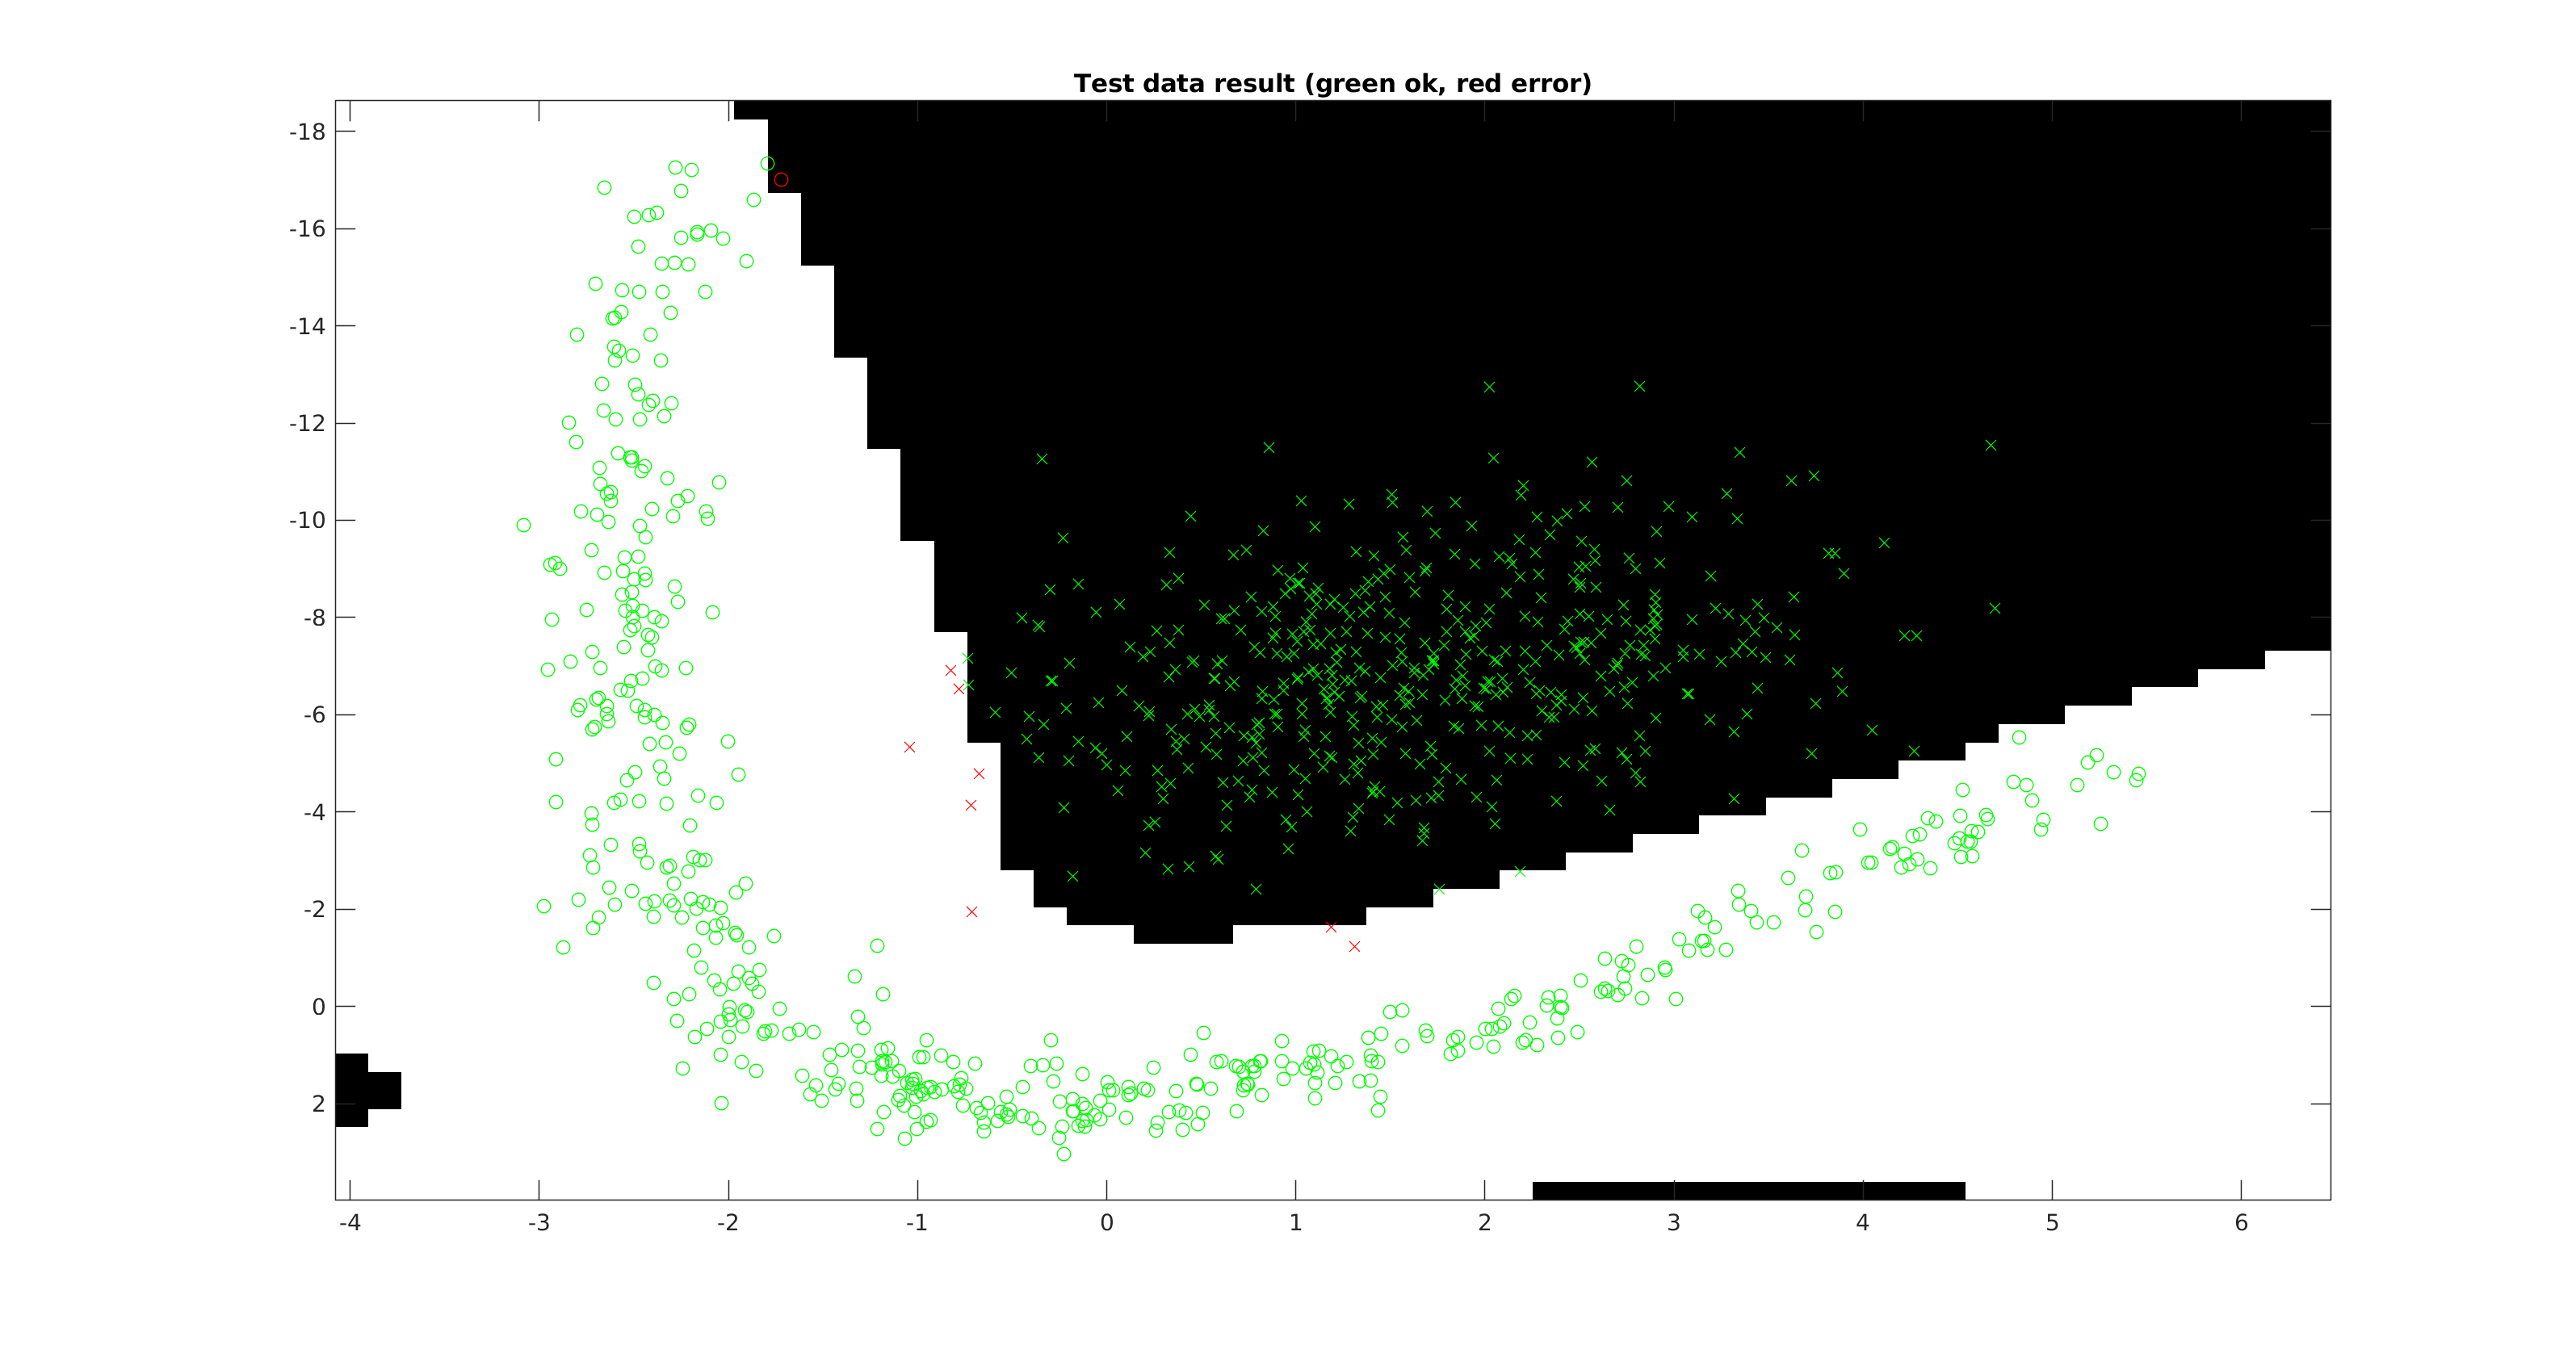
\includegraphics[width=13cm]{dataset2res.png}
    \caption{Results for dataset 2}
    \label{fig:res2}
\end{figure}

\subsection{Dataset 3}

A multi-layer network with 20 hidden neurons was used here, trained with 12 000
iterations at a learning rate of 0.004. Many iterations were used here, since
both the training error and testing error kept decreasing for quite a while
until it stopped improving.

For the other datasets we chose a multi layer network because they
require a non linear classifier.

Figure~\ref{fig:res3} shows the result of this.

\begin{figure}[h!]
    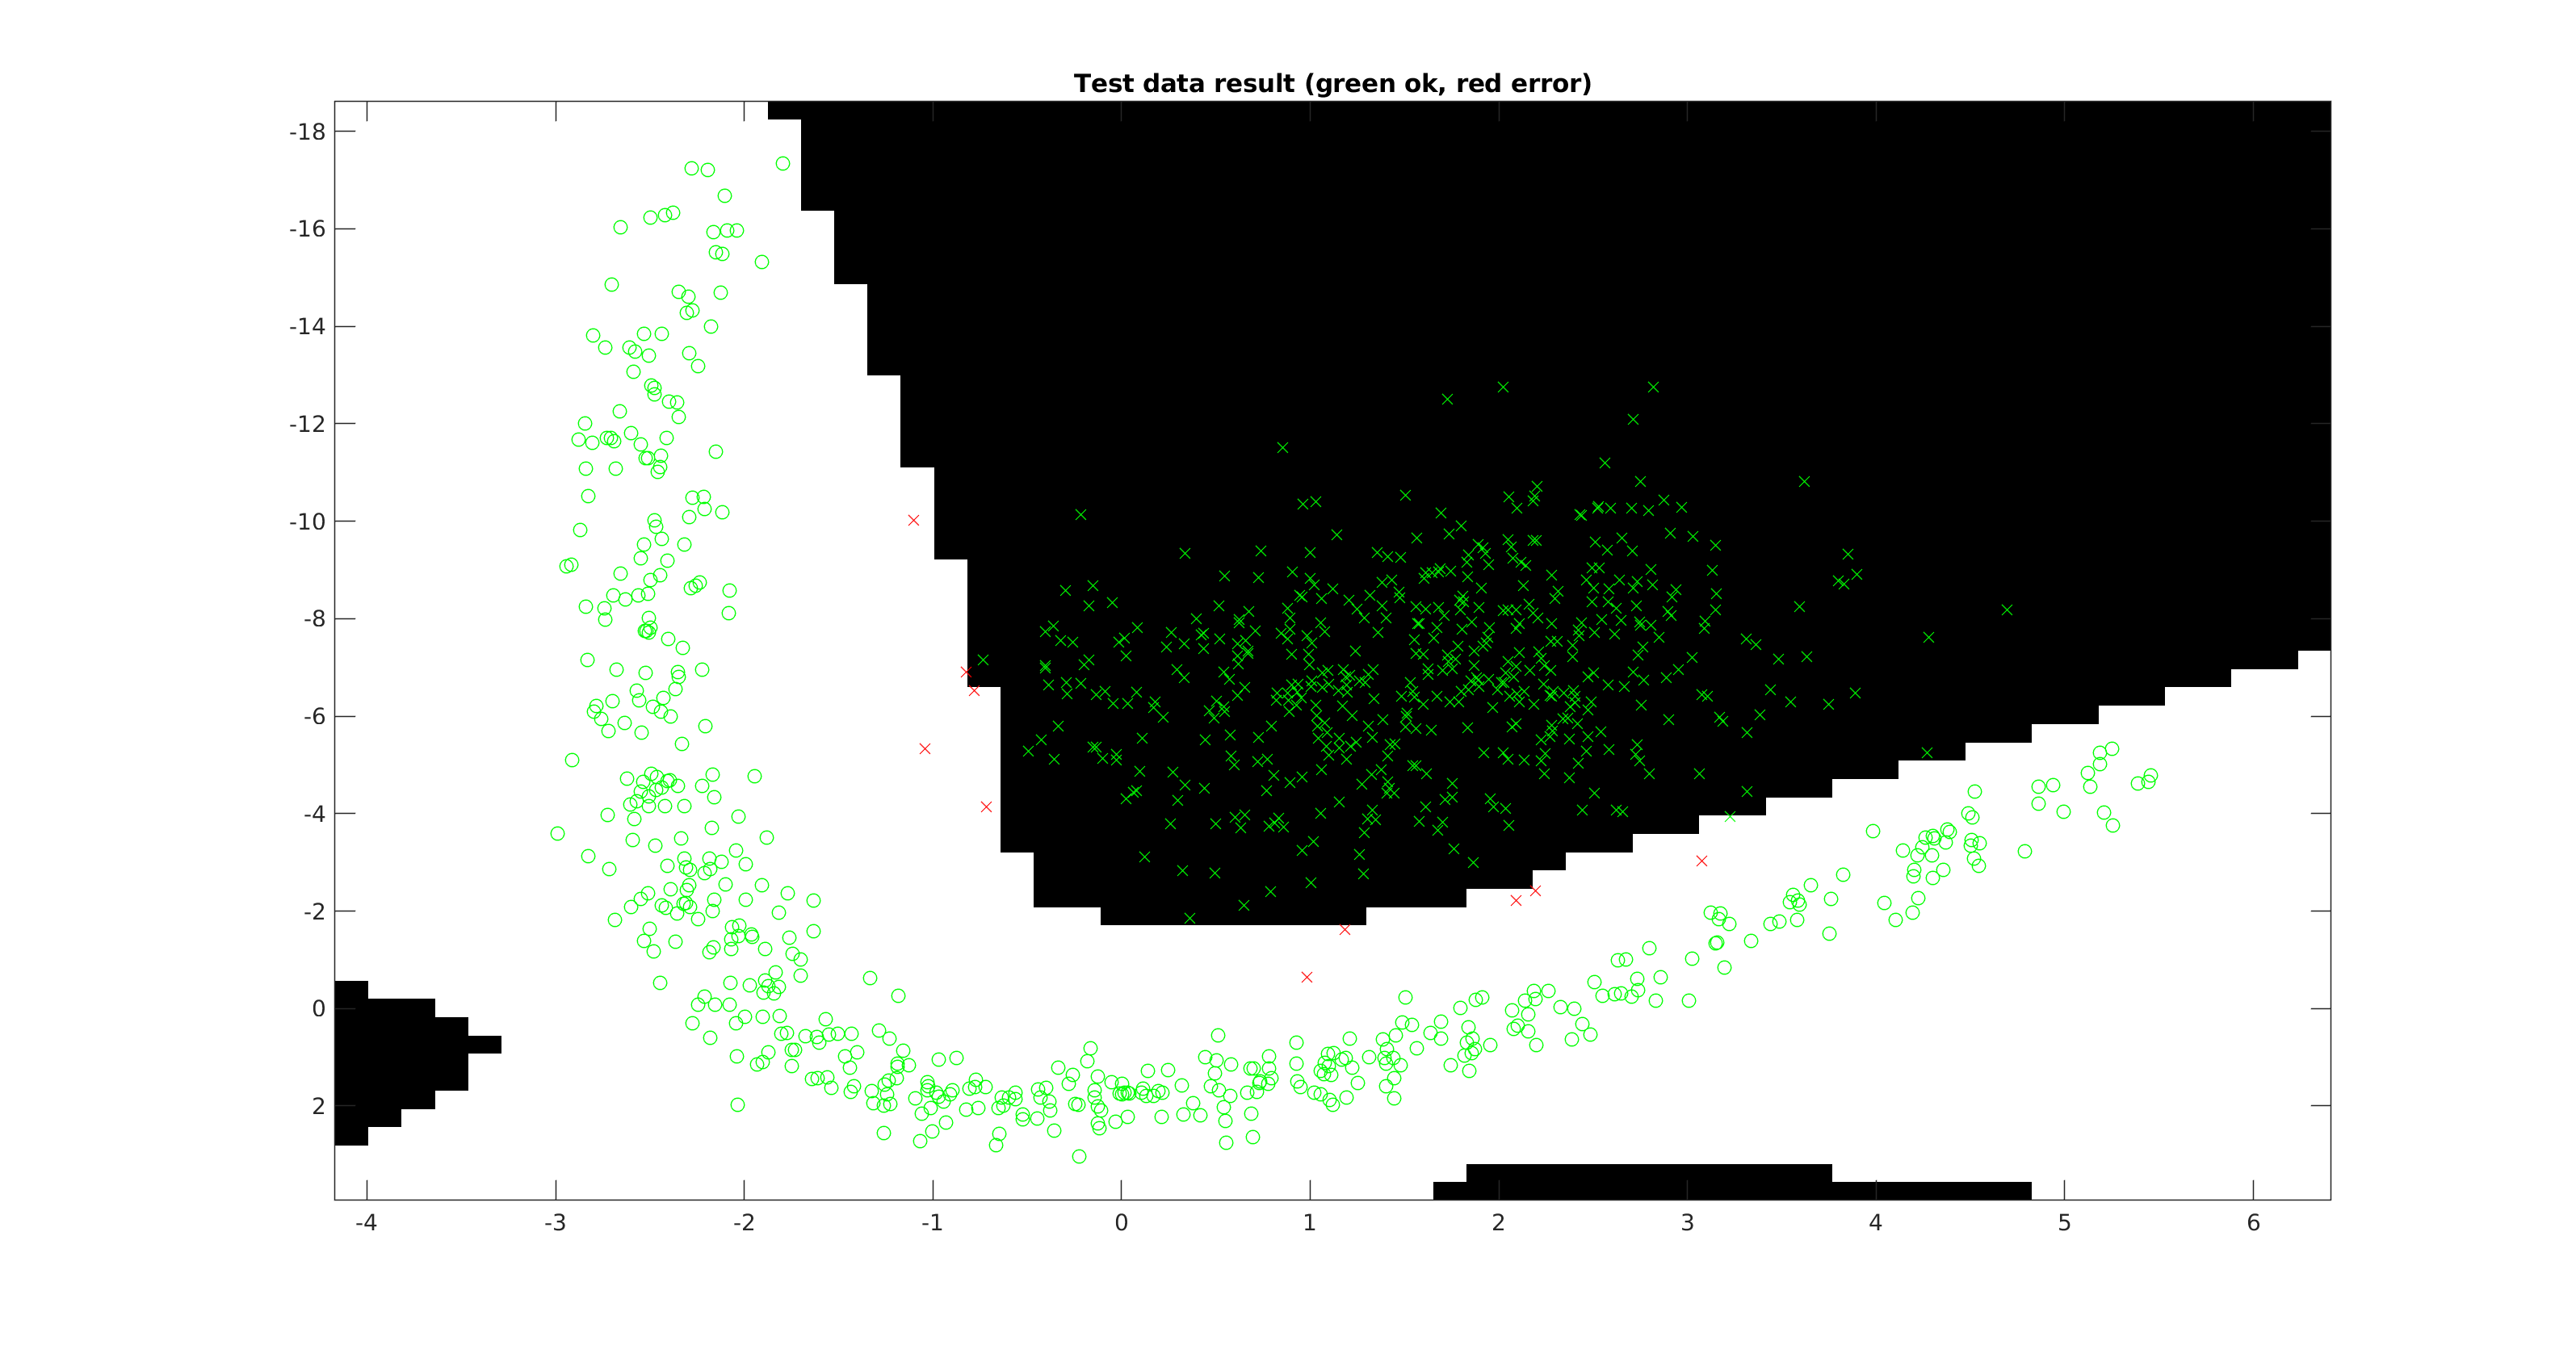
\includegraphics[width=13cm]{dataset3res.png}
    \caption{Results for dataset 3}
    \label{fig:res3}
\end{figure}

\subsection{Dataset 4}

Again, a multi-layer network was used here. Due to the high dimensionality of
the input space, 100 hidden neurons was used. The number of
iterations did however not need to be higher than 4000, since the test error
did not get much smaller beyond this point, and the network already took quite
a long time to train.

Figure~\ref{fig:res4} shows the result of this.

\begin{figure}[h!]
    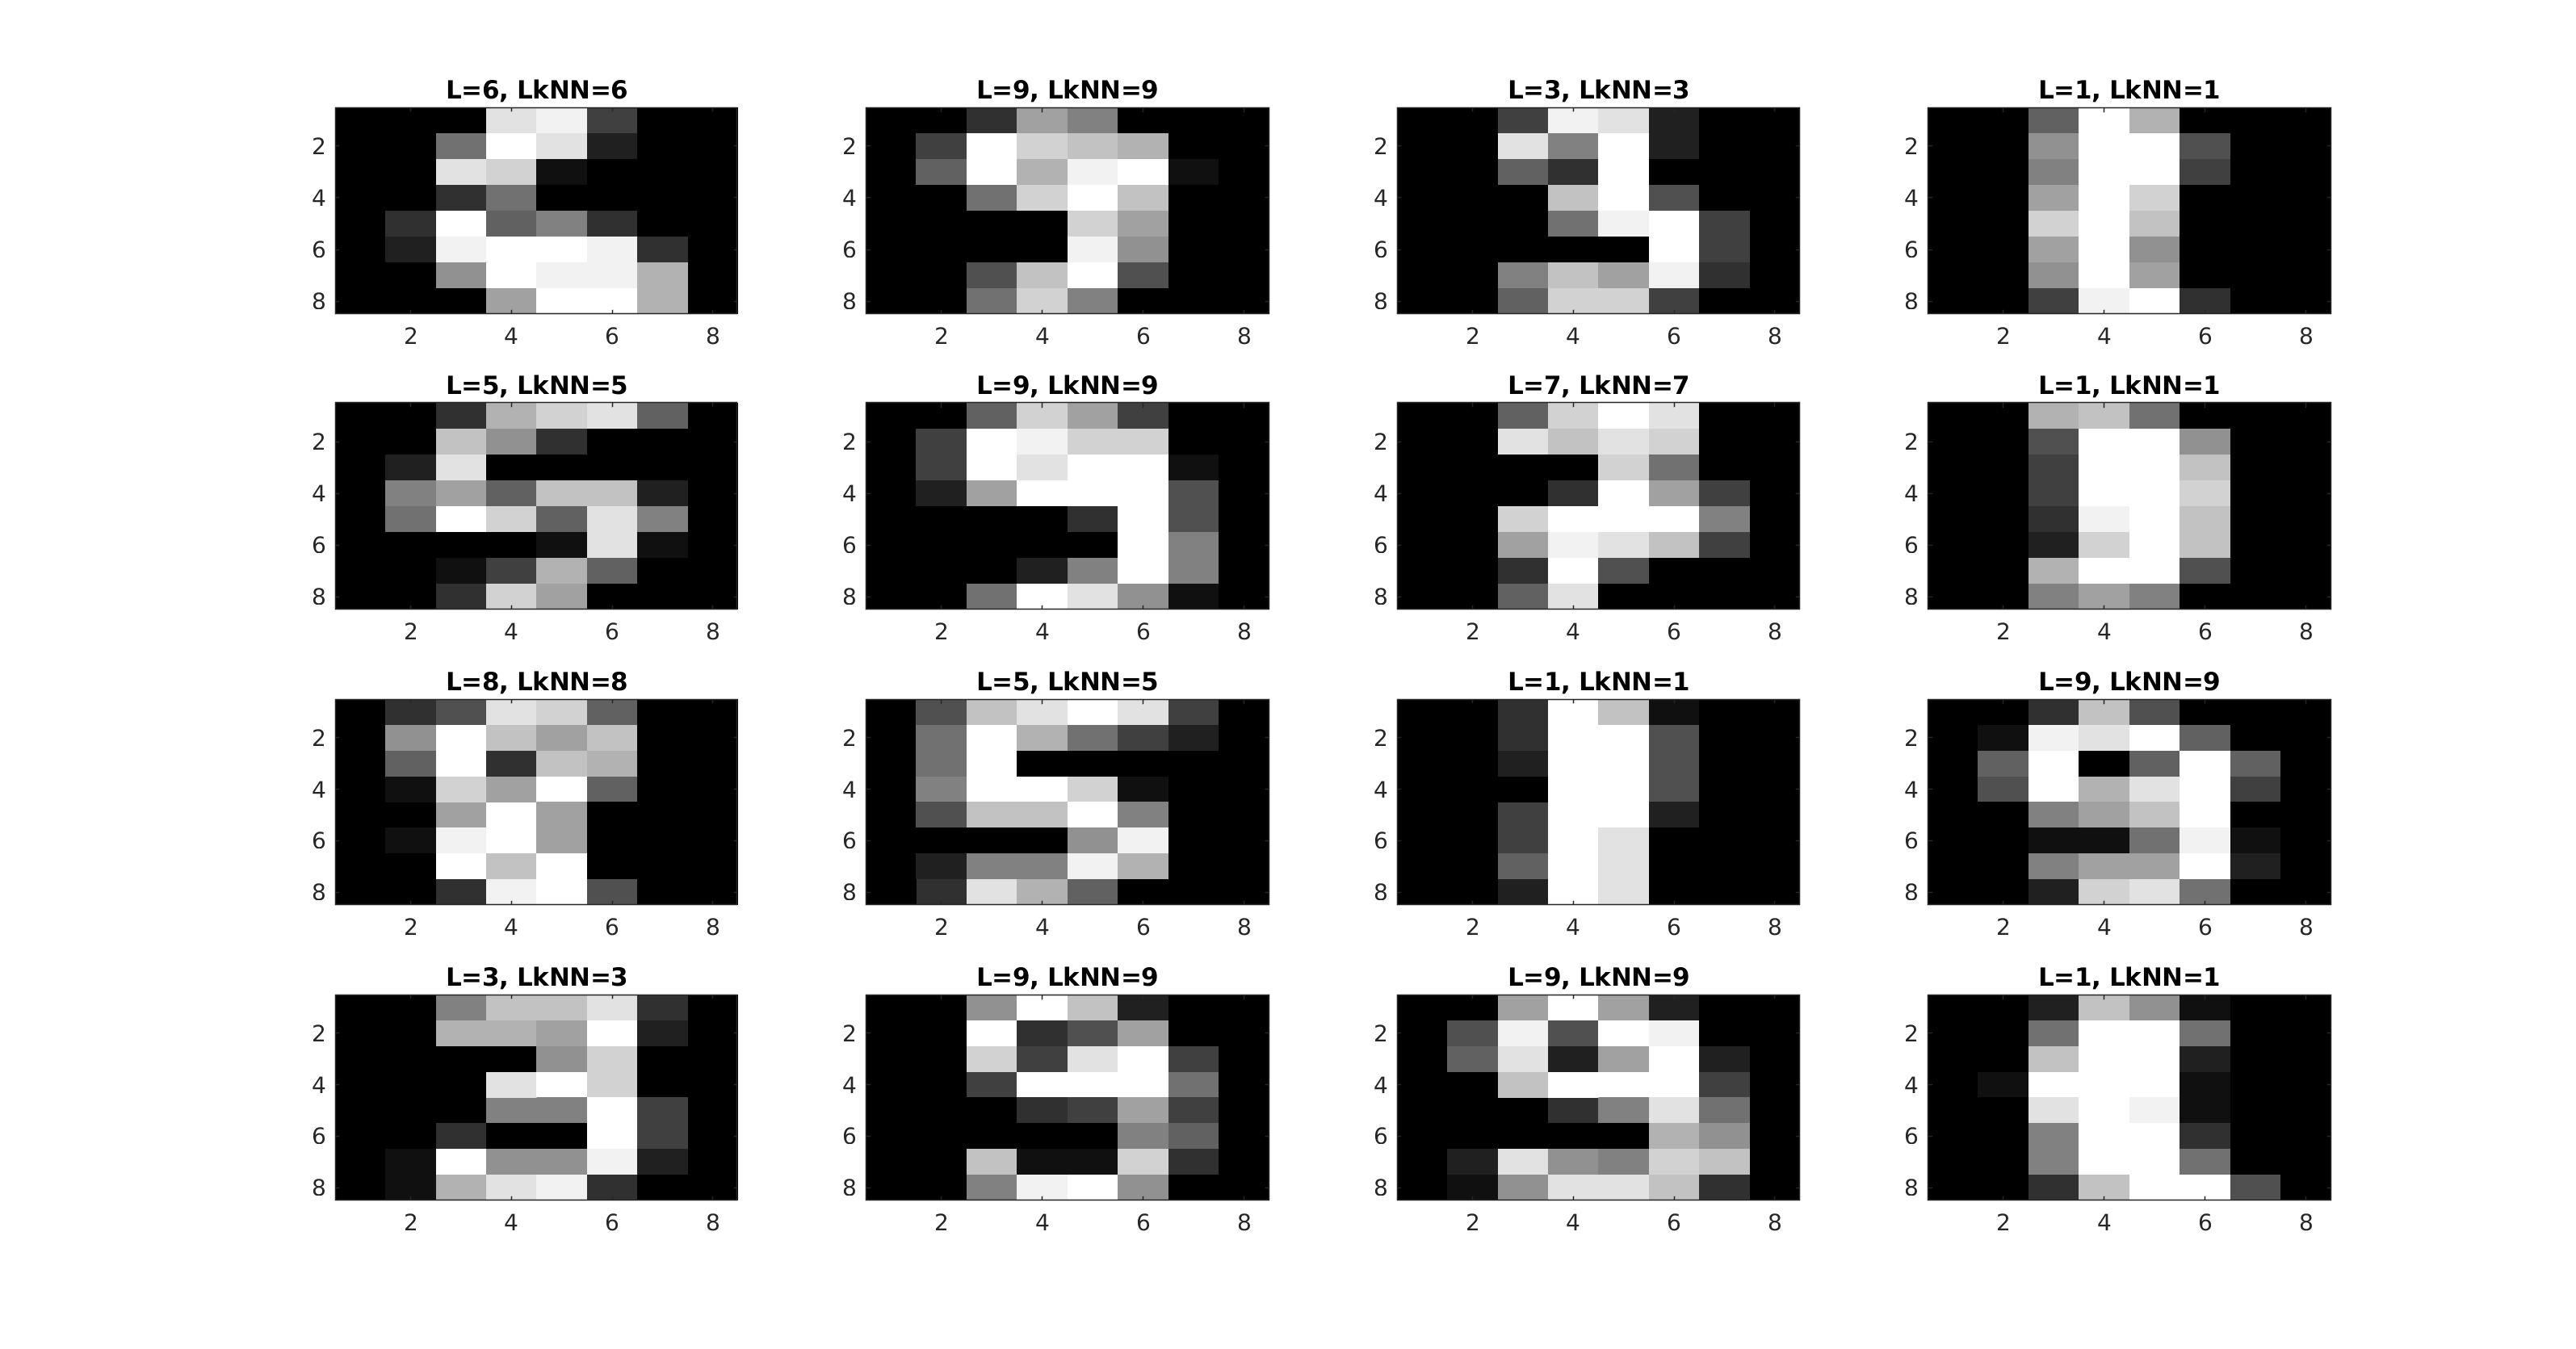
\includegraphics[width=13cm]{dataset4res.png}
    \caption{Results for dataset 4}
    \label{fig:res4}
\end{figure}

\section{Non-generalizable solution}

To generate a non-generalizable solution for dataset 3, the number of training
examples was reduced to 10. This caused the test error to not decrease as the
training error decreased, as seen in Figure~\ref{fig:errornongen}, since the
network is over-fitted to the little data it has available. The fact that the
data also only contains examples of one class further makes it so that it has
no reason to not classify everything as one class. This can be seen in 
Figure~\ref{fig:trainnongen}, where it correctly classifies the few training
examples. However, this of course doesn't generalize well to examples it hasn't
seen before, as shown in Figure~\ref{fig:testnongen}.

\begin{figure}[h!]
    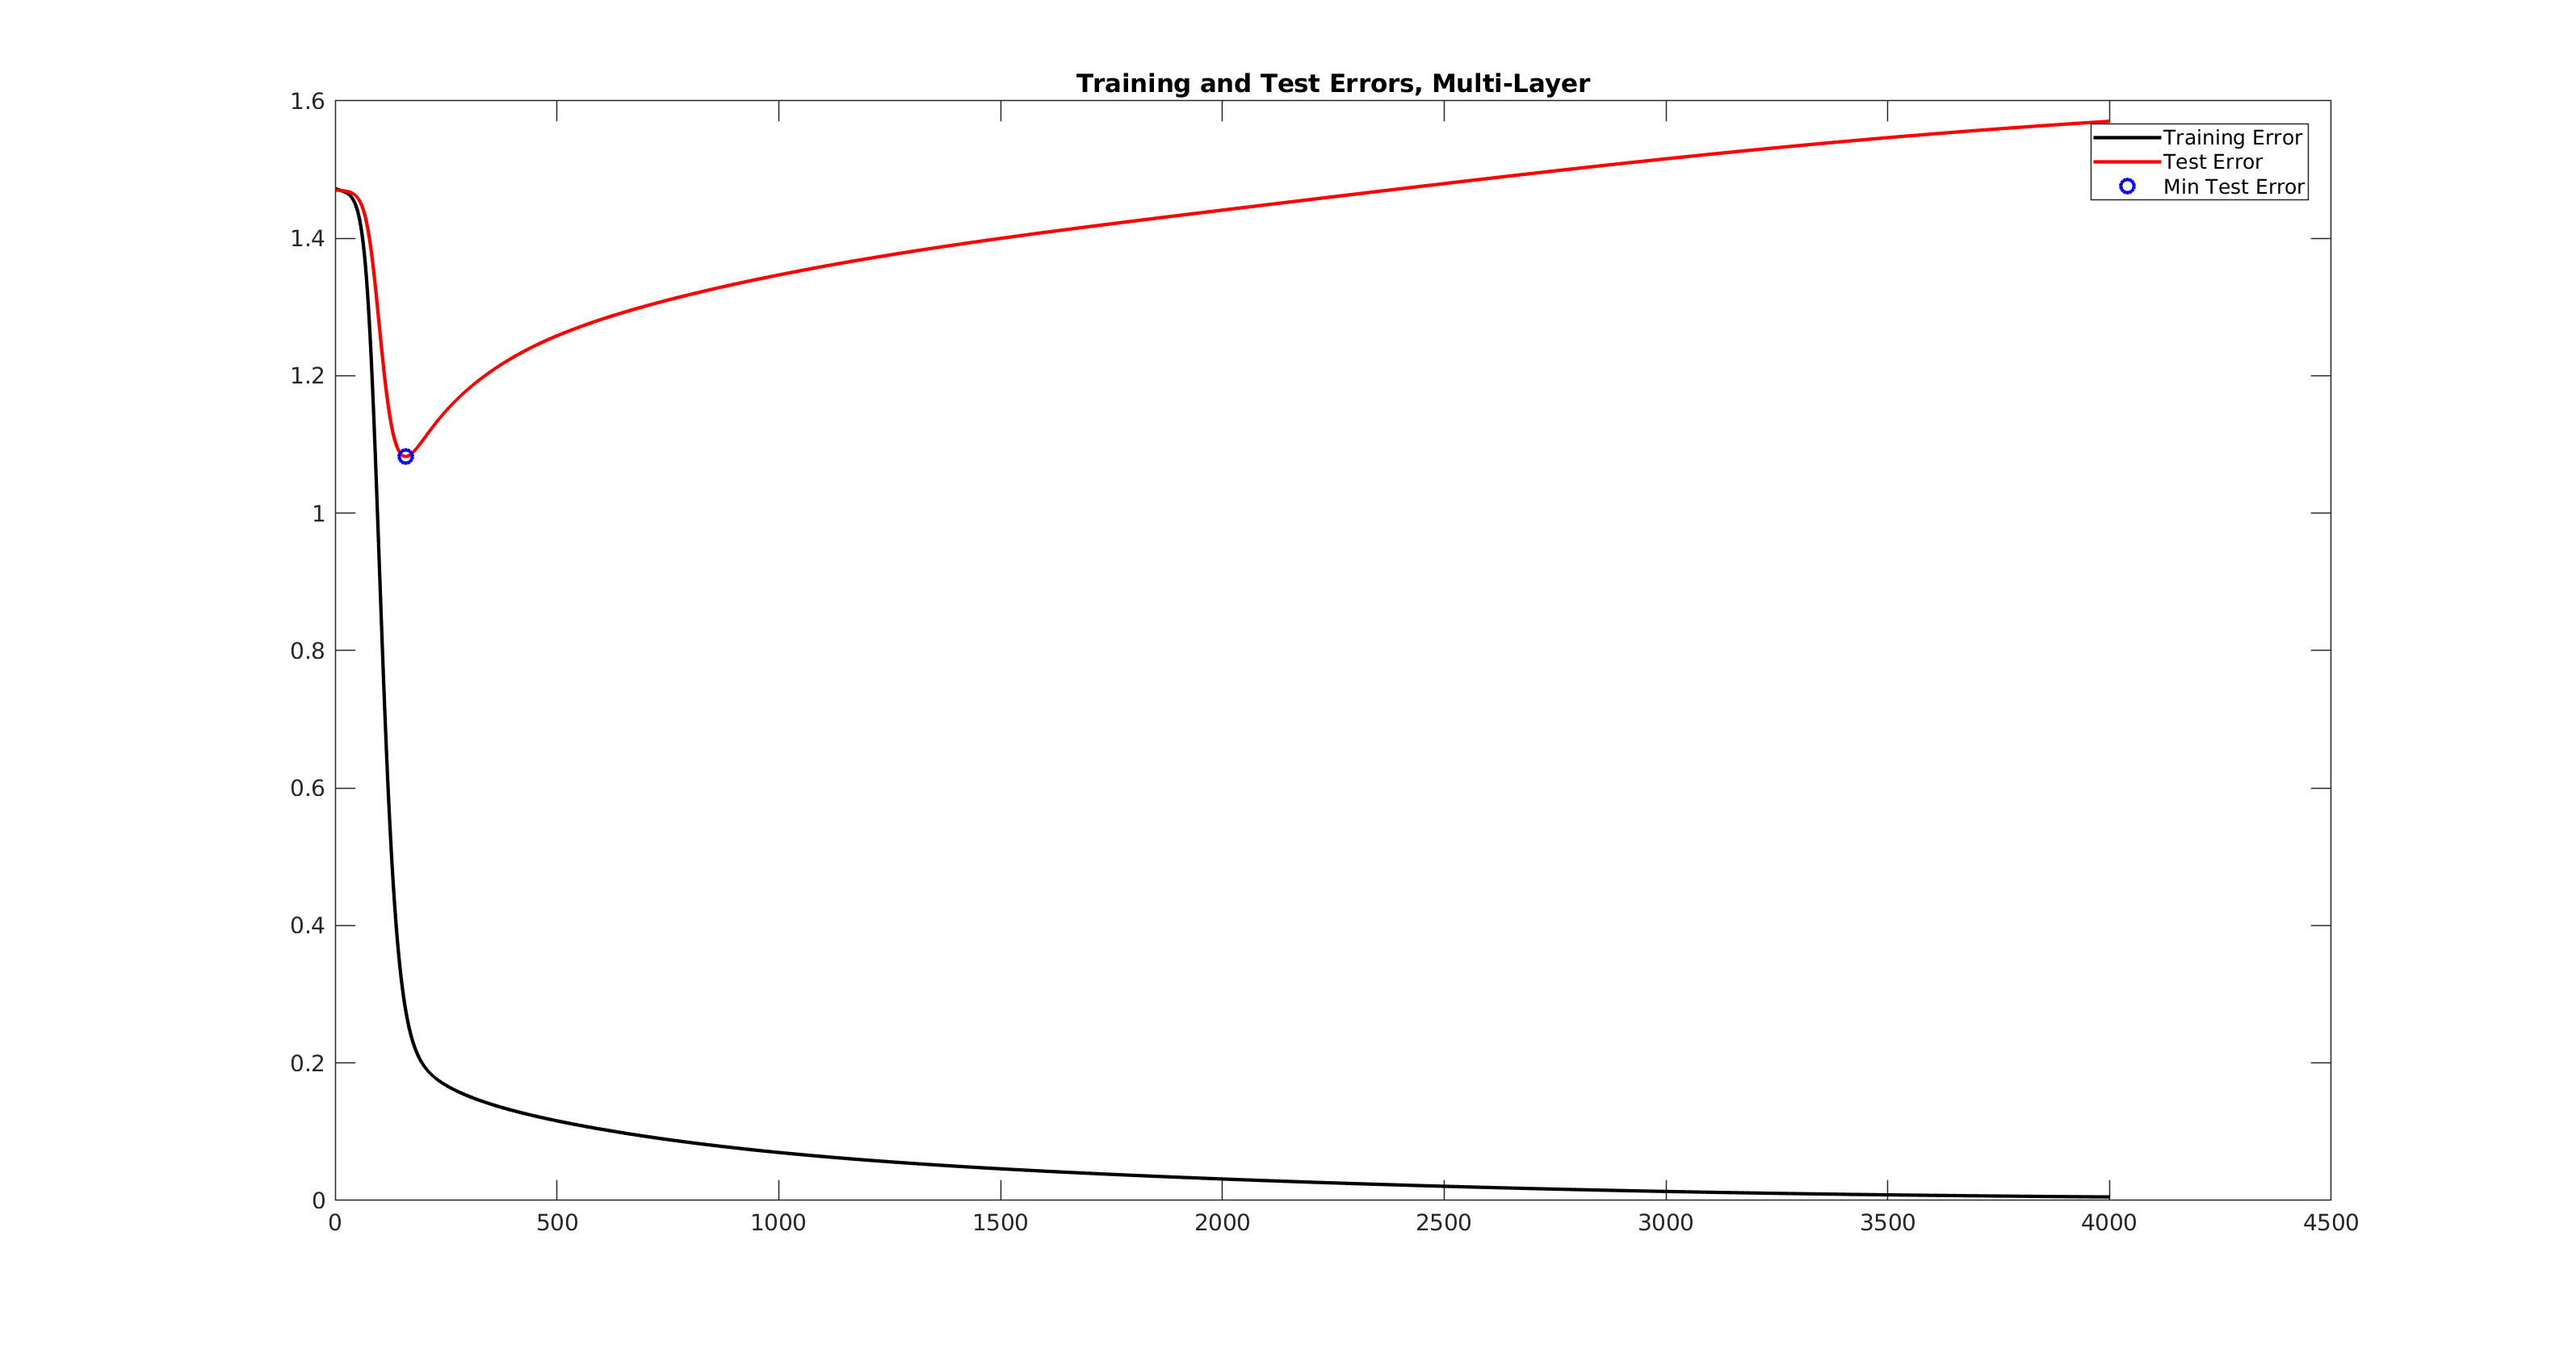
\includegraphics[width=13cm]{errornongen.png}
    \caption{Plot of errors for non-generalizable solution}
    \label{fig:errornongen}
\end{figure}

\begin{figure}[h!]
    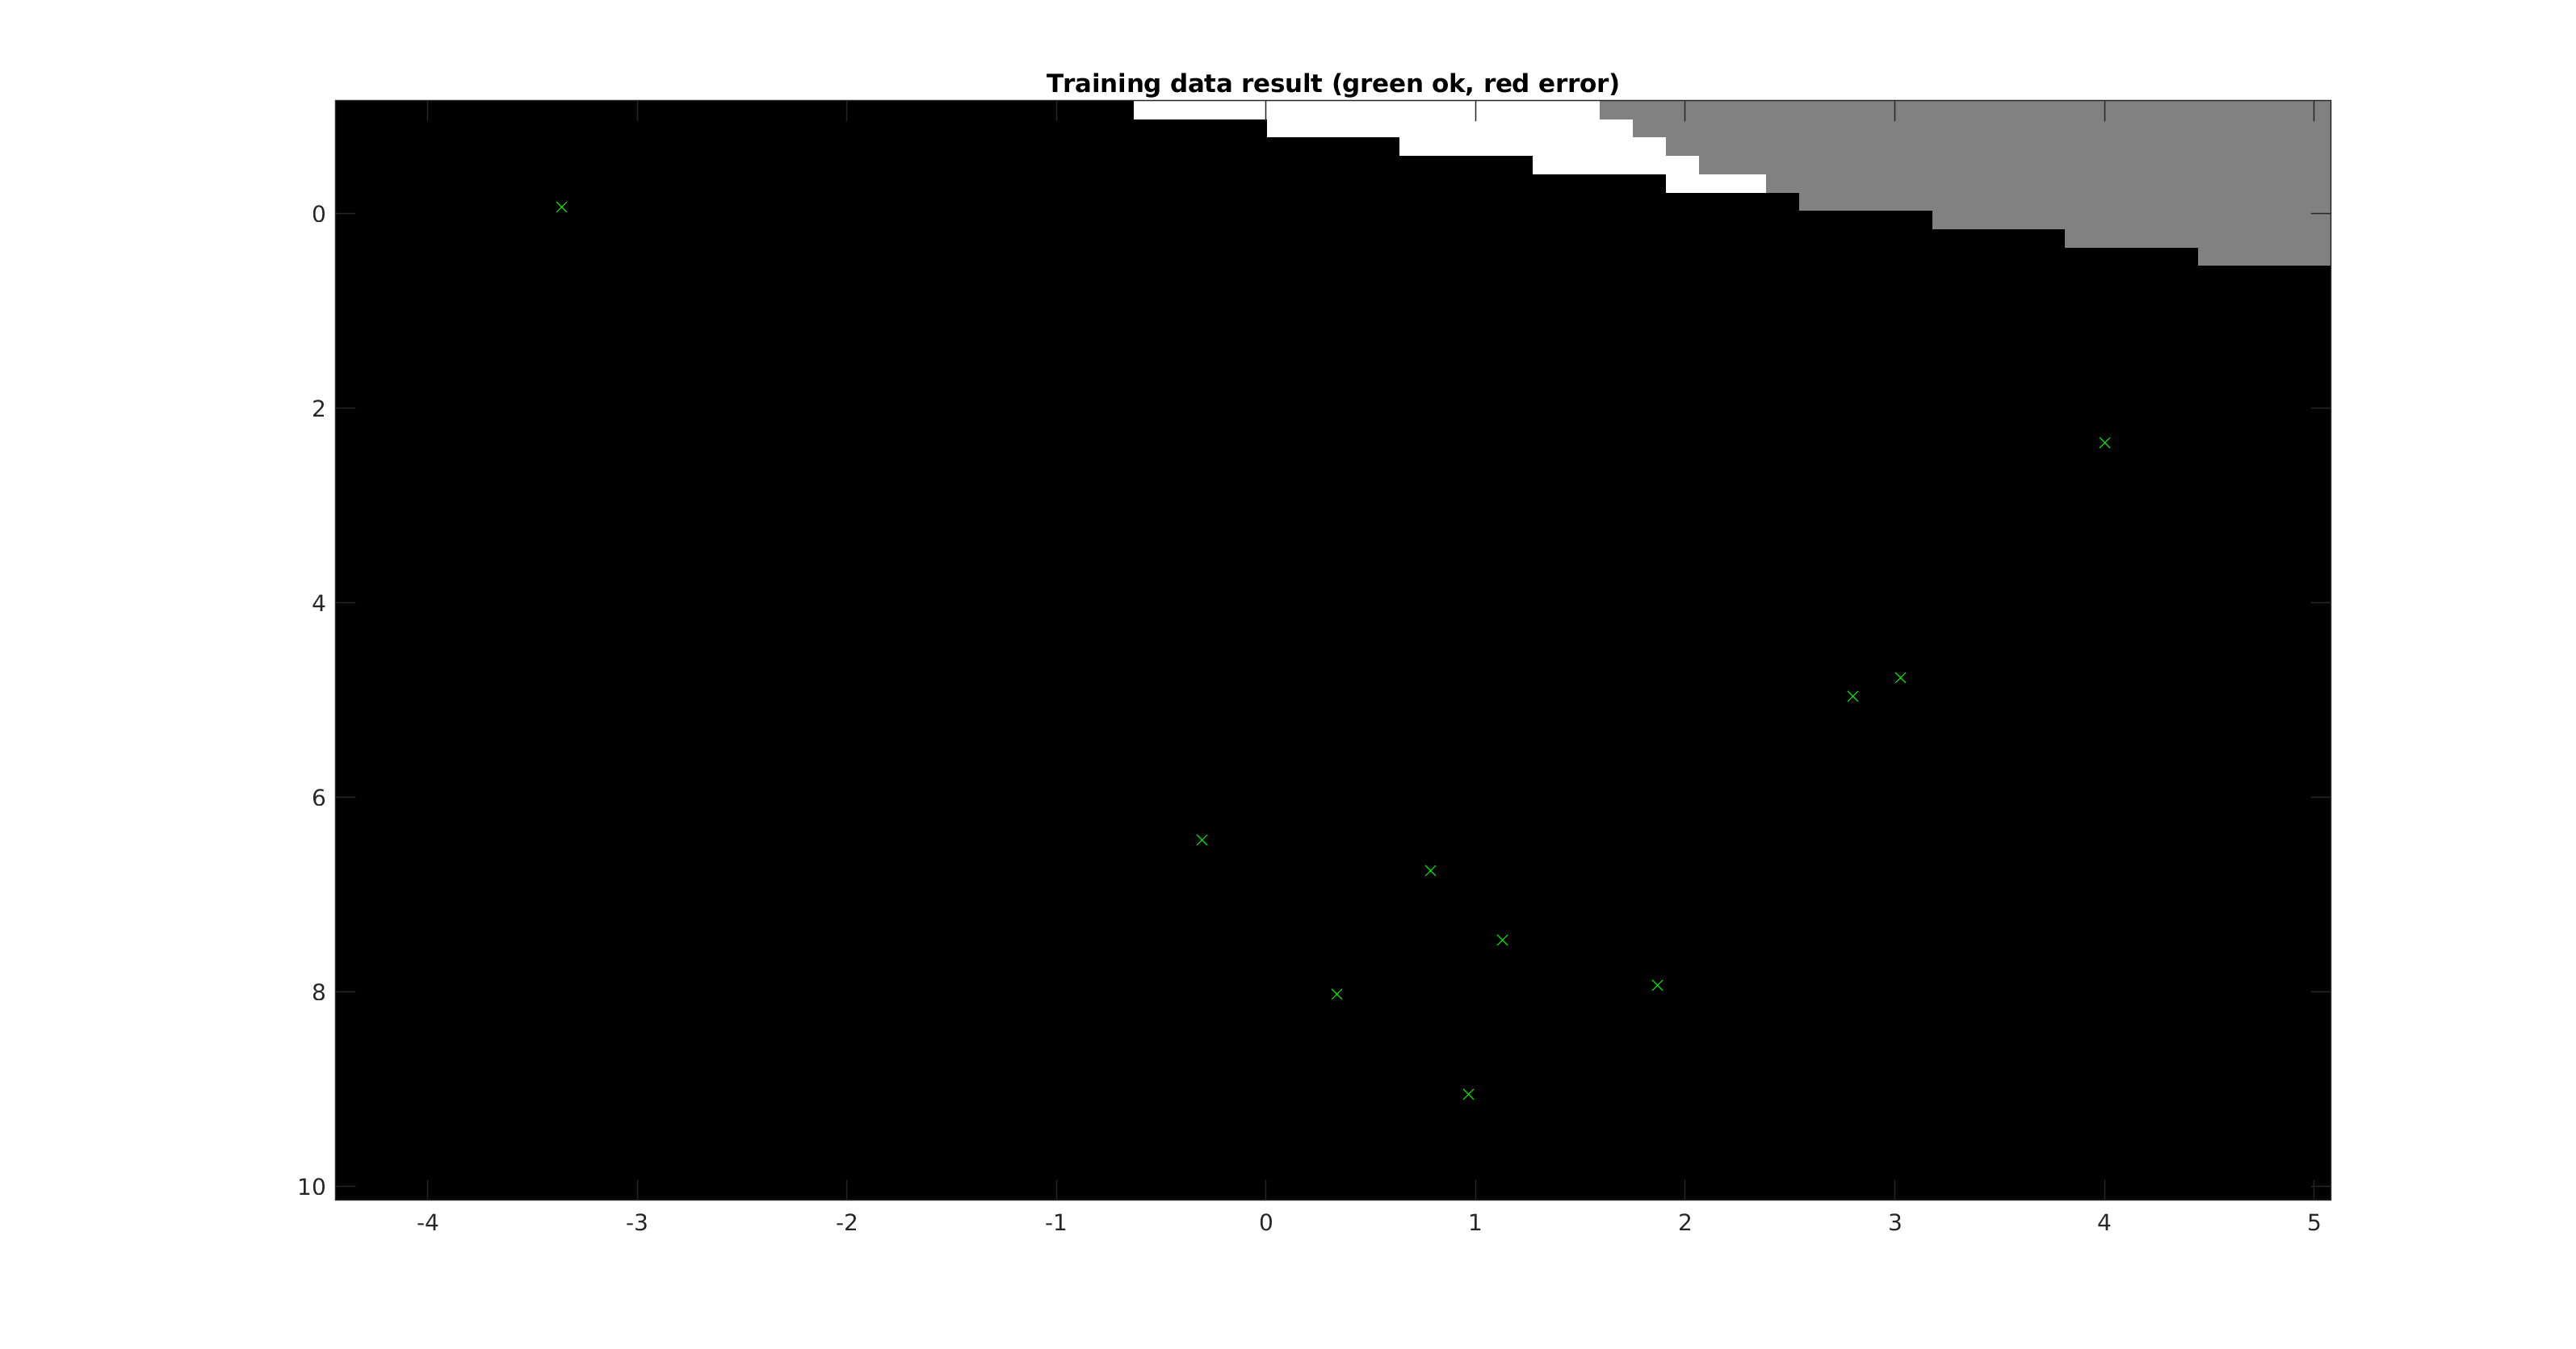
\includegraphics[width=13cm]{trainingresnongen.png}
    \caption{Training results for non-generalizable solution}
    \label{fig:trainnongen}
\end{figure}

\begin{figure}[h!]
    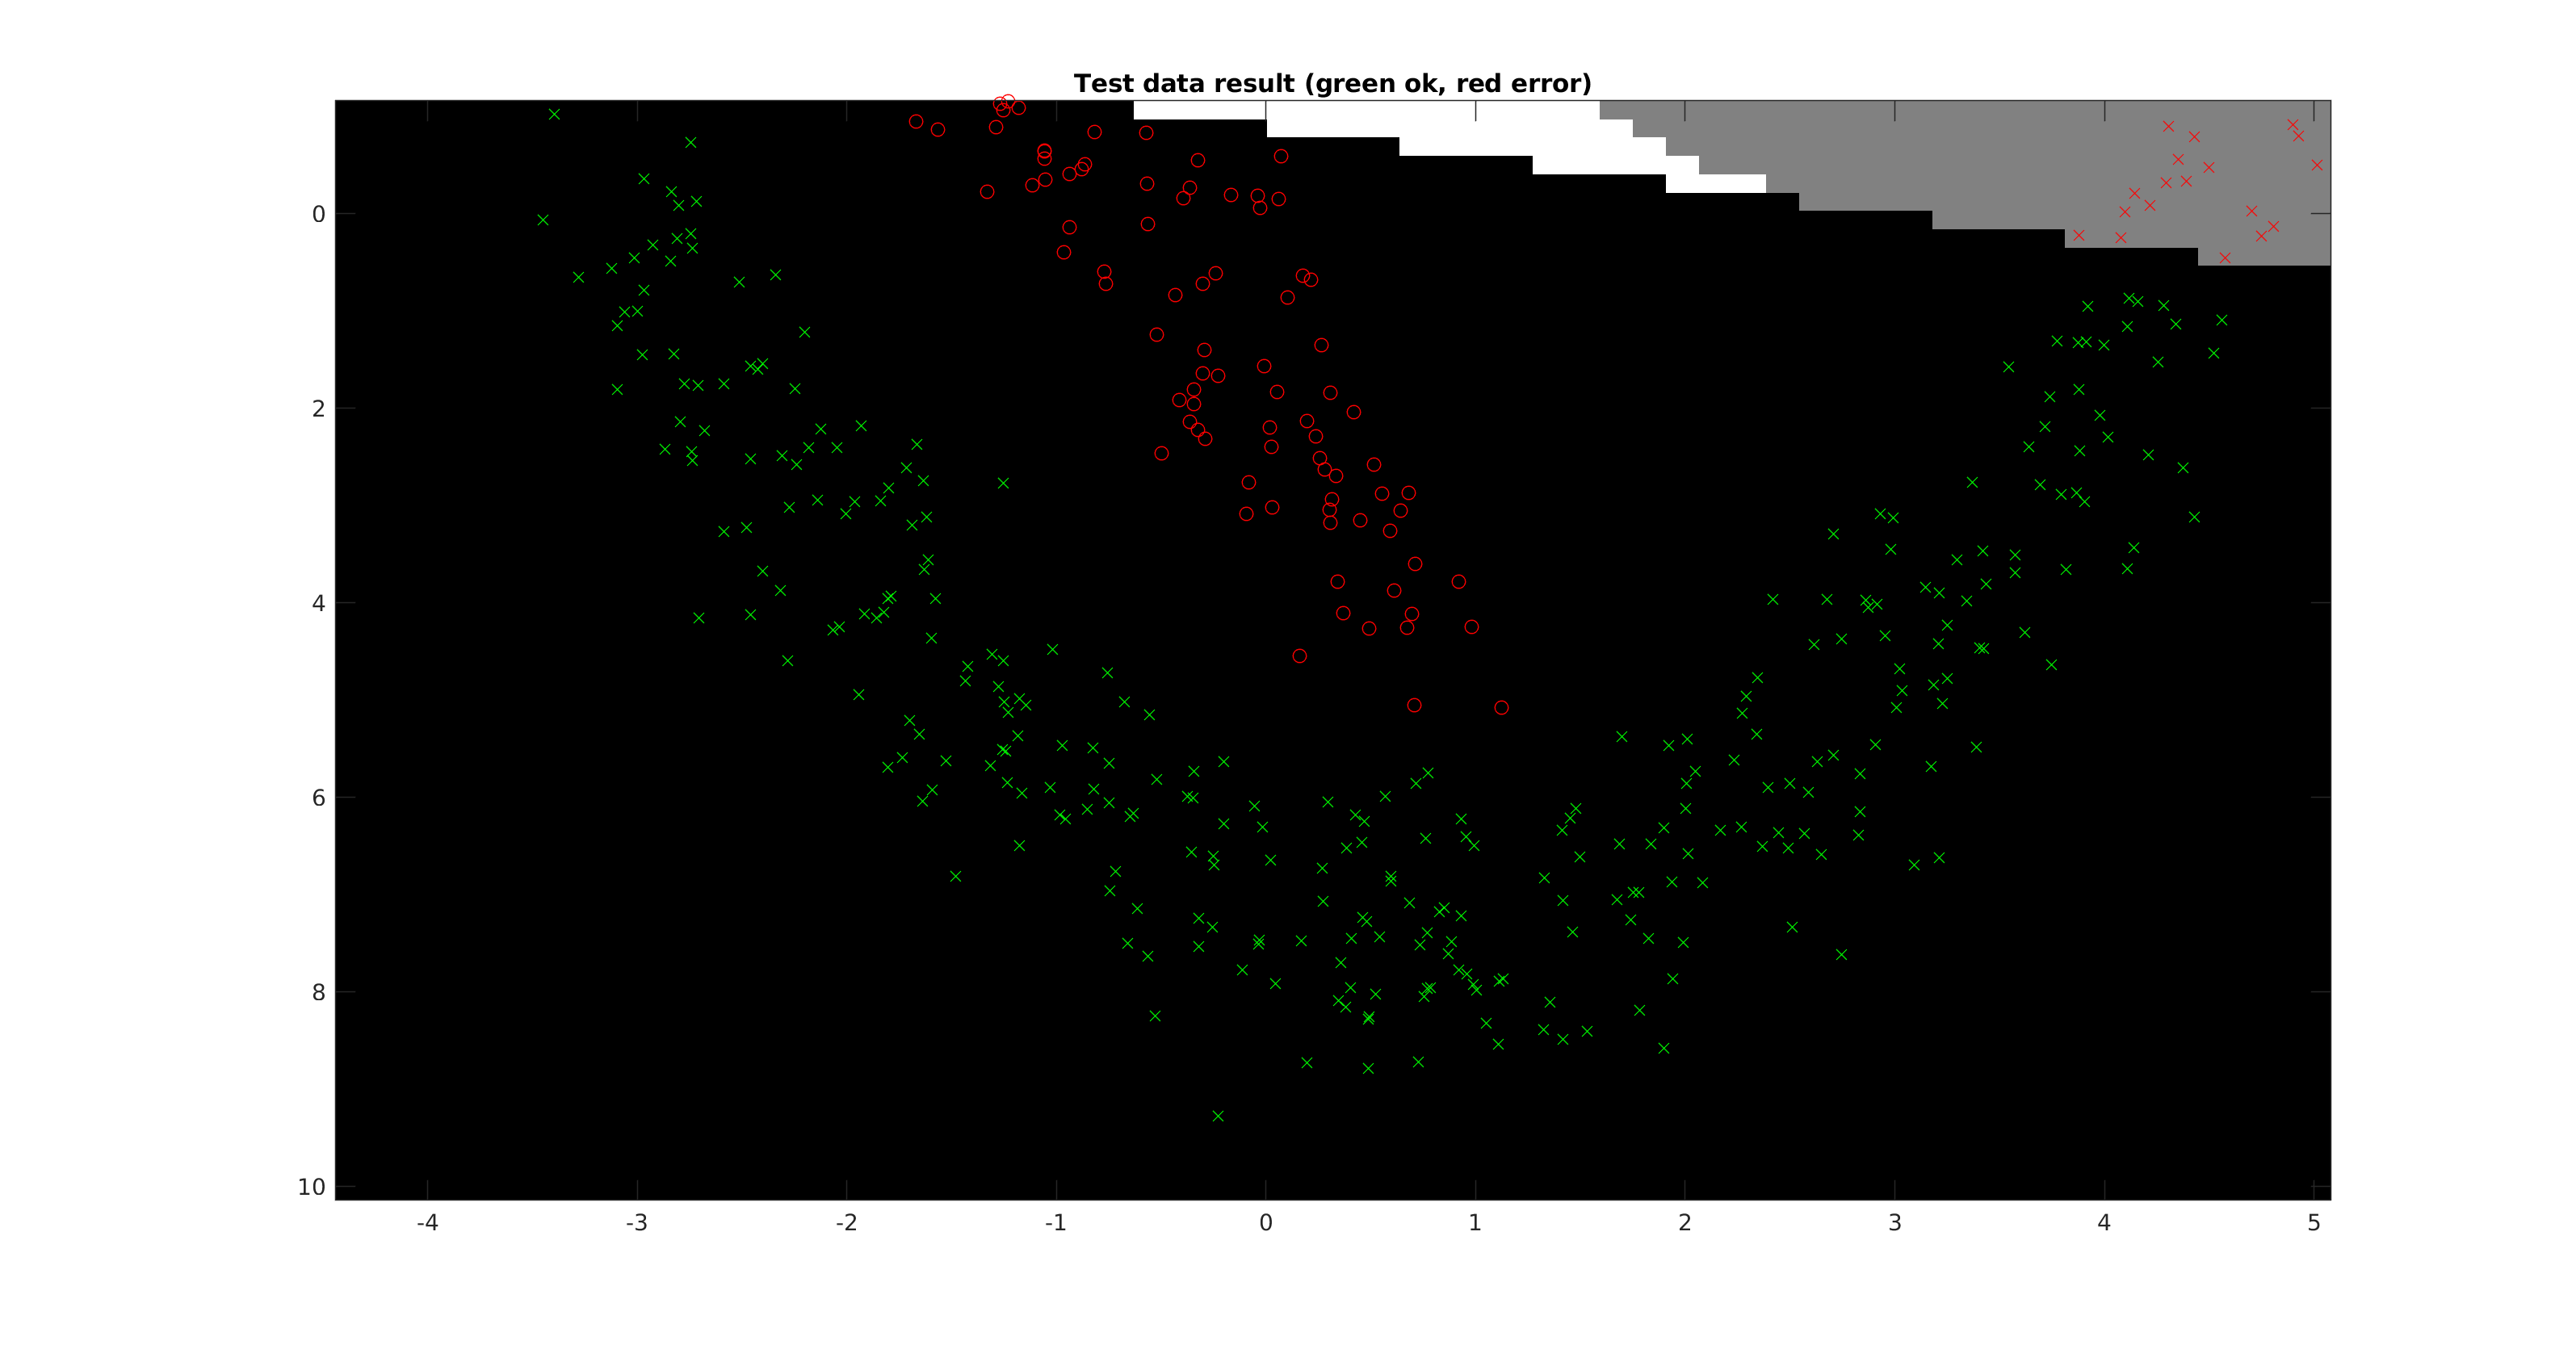
\includegraphics[width=13cm]{testresnongen.png}
    \caption{Test results for non-generalizable solution}
    \label{fig:testnongen}
\end{figure}

\section{Discussion}

kNN gives very good performance on all datasets, and is fast to evaluate with
small datasets. No
training is required either. The downside of kNN is however that you need
access to all ``training'' examples when evaluating a new sample, which can be
impractical if the problem requires a large number of examples.

With single layer network, one does not need to store all training examples,
only the weights need to be stored. It gives good performance on linearly
separable problems, but it can't handle more complex problems or the
XOR-problem.

A multi-layer network gives good performance on simple and complicated
problems, and unlike kNN, the training examples need not be stored, only
the weights. The downside of a multi-layer is, however, that it can take
a long time to train it.

\section{Possible improvements}

One way section improve the performance and training time of the multi-layer
network would be to introduce a momentum term 
$\alpha\Delta w_{ij}(t - 1)$ in the gradient descent, such that the step
length is affected by the lenght of the step before. That is, if the
sign of the derivative is the same for some time, the step length
increases, otherwise it decreases. This will give faster convergence
and decrease the risk of ending up in a suboptimal local minimum of the
cost.

\end{document}
